\documentclass[a4paper,10pt]{article}
\usepackage[margin=2.5cm, nohead]{geometry}
\usepackage{palatino, url, multicol}
\usepackage{graphicx}
\usepackage{verbatim}
\usepackage[all]{xy}
\usepackage[english]{babel}

\newcommand{\bits}{BITS}
% The current value of the timeThreshold given to awesomizeClusters.
\newcommand{\timeThreshold}{1200}

\title{Leren en Beslissen - ACHTBITS\\\large \textsc{Awesome Charadriiformes Toegepast
BIrd Tracking System}}
\author{Maarten de Waard\\5894883 \and Maarten Inja \\5872464 \and Jesse Eisses \\
6352189 \and Sosha Happel\\ 6273831}



%\email{mrtndwrd, maarten.inja, jesse.eisses, soshappel@gmail.com}
\begin{document}
\maketitle
\begin{abstract}
Of course we will have an abstract! But we can't type this yet, because we don't
know the results. And everybody knows abstracts have spoilers! Also Dumbledore
gets killed by Snape.
\end{abstract}
\section{Introduction}
% I guess we will introduce the BITS, introduce some other stuff, maybe tell
% something about learning algorithms in general

\section{Preprocessing}
% Here we will discuss the preprocessing of the .csv files. This should consist
% of:
 \subsection{Getting the data we need}
 % Describing how we only get the data above the north sea. Maybe an appendix
 % should be added on how the java script can (should) be run.
 
 \subsection{Finding clusters in the data}
 % Describes how we find the peaks/clusters in the data (Maarten de Waard will
 % fill this in)
 This section will discuss how we find clusters in the raw data. 
 This is needed, to annotate these clusters, so we can later on use a
 learning algorithm on specified parts of the data.

 Probably the most important of the GPS data we get from \bits are the X and Y
 position and speed of the bird. There are two speed entries in the database we
 use: One `instantaneous speed', the speed the bird has on the time of
 connecting to the GPS, calculated from two subsequent measurements, and a
 `trajectory speed', the speed the bird has between this, and the last
 measurement point. For clustering, we decided to use the latter, because this
 has a smaller error rate. Our assumption is that we can cluster the data good
 enough, by only looking at speed differences. Figure \ref{fig:speeds} shows
 why.
 % TODO: Dit figuurtje maken. Ik kom er namelijk net achter dat de derivative
 % misschien niet exact doet wat we willen, omdat het speed1 en speed2 apart van
 % elkaar gebruikt. Een goeie hiervoor is device_535, sessie_000.
\begin{figure}
\centering
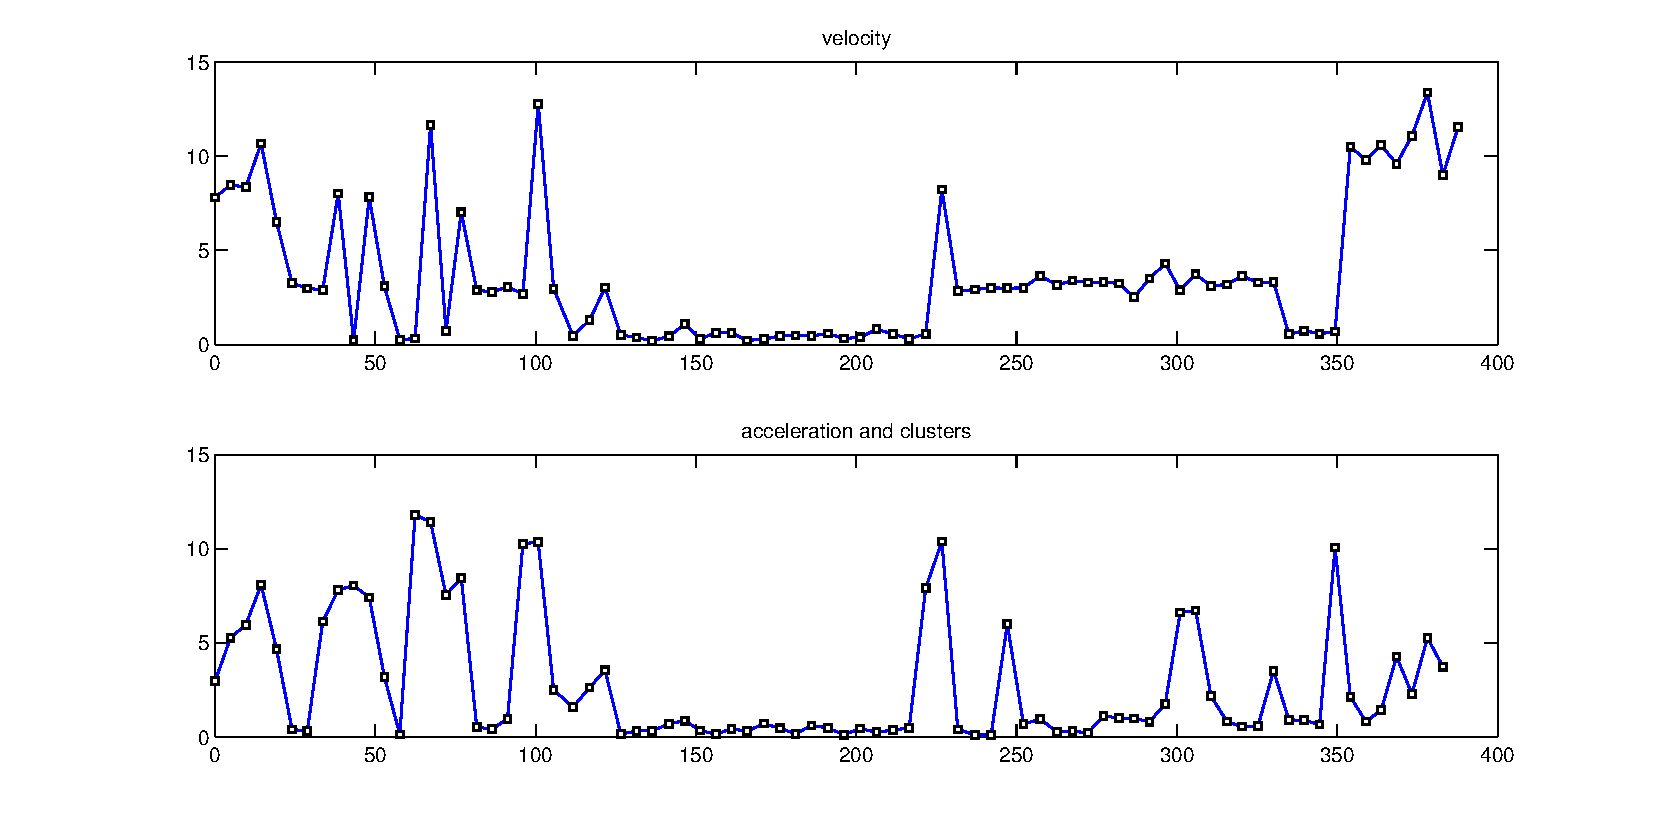
\includegraphics[width=.8\textwidth]{speed.pdf}
\caption{The speed of the bird (above) and the difference in speed (under). As
you can see, the difference is absolute (because this makes finding peaks
easier). The difference is some times a bit higher, while the speed does not
seem to differ at all. This means the bird changed his direction.}
\label{fig:storyboard}
\end{figure}

 As can be seen, the speed-difference is low on points where the bird is assumed
 to be flying or sitting on the water. In other points the speed differs a lot.
 On these places we can assume that the bird is foraging.

 \subsubsection{Finding peaks}
 Clustering, in our case, starts with finding peaks in these speed differences.
 The peaks indicate a change in the bird's behavior, or indicate that the bird
 is foraging. Finding these peaks is done in two steps:

 \begin{itemize}
    \item Check where the value of the speed difference is bigger than a certain
    threshold.
    \item Loop through these differences and place a marker before the threshold
    is crossed upwards, or after it has been crossed downwards. 
 \end{itemize}
 
 This creates a representation of a peak by marking its left and right side.
 This comes in handy, because we do not want these speed differences in our
 clusters as they would add noise to the learning data.

 \subsubsection{Grouping peaks}
 For grouping peaks, we created another algorithm. This algorithm looks at three
 characteristics.  
 \begin{enumerate}
 \item The time elapsed between two peaks
 \item The difference between the current time elapsed between peaks, and the
 current cluster's average
 \item The difference between the time elapsed between the first peak of the
 cluster, and the average of the rest of the cluster.
 \end{enumerate}
 This way we can find the `chaos clusters', because the time between the peaks
 in these clusters is always between a certain threshold (currently set on
 \timeThreshold seconds). 
 When a peak is too far from the  current average, this almost always indicates
 a change in behavior, so a new cluster should be started.this is done by the
 second and third characteristic specified above.


 \subsection{Annotating the data}
 % Describes how we annotate (including how the tool works. Maybe an appendix
 % should be added on how the tool should be started and how it should be used.


\section{Learning}

\section{Conclusions and results}

\section{Improvements and future work}


\end{document}
